\ifdefined\COMPLETE

\else
\documentclass[journal=langd5,manuscript=article]{achemso}
%\usepackage[margin=1in]{geometry}
\usepackage{rotating}
\usepackage[T1]{fontenc}
\usepackage[utf8]{inputenc}
\usepackage{flafter}
%\usepackage{floatflt}
\usepackage{placeins}
\usepackage{siunitx}
\usepackage{graphicx}
\graphicspath{{./figures/}}% Include figure files
%\usepackage{epstopdf}
\usepackage{dcolumn}% Align table columns on decimal point
\usepackage{appendix}
\usepackage{amsmath}
\usepackage{commath}
\usepackage{cases}
\usepackage{calc}
\usepackage{amssymb}
\usepackage[dvips]{color}
\usepackage{color}
\usepackage{enumitem}
\usepackage{soul}
\usepackage{indentfirst}
\usepackage{hyphenat}
\usepackage{xspace}
\usepackage{subcaption}
\usepackage{booktabs}
\usepackage{multirow}
\usepackage{tabularx}
\usepackage{xcolor}
\usepackage{lineno}
% \usepackage{hyperref}
\usepackage{setspace}
\usepackage[draft,xcolor=dvipdf]{changes}
\usepackage{mciteplus}
\newcommand{\tbxmulticol}[3]
    {\multicolumn{#1}
                 {>{\centering\hsize=\dimexpr#1\hsize+#1\tabcolsep+\arrayrulewidth\relax}#2}
                 {#3}}
\newcommand{\ra}[1]{\renewcommand{\arraystretch}{#1}}
%\newcommand{\cmpersec}{$\frac{\text{cm}}{\text{s}}$~}
\newcommand{\cmpersec}{cm/s~}
\newcommand{\etal}{\textit{et al.}~}
\newcommand{\na}{Na\textsuperscript{+}~}
\newcommand{\cl}{Cl\textsuperscript{-}~}
\newcommand{\li}{Li\textsuperscript{+}~}
\newcommand{\mg}{Mg\textsuperscript{2+}~}
\newcommand{\mbnbfix}{MB-NB-fix~}
\newcommand{\mbnbfixmicro}{Grotz \etal~}
\newcommand{\nambnbfix}{Na\textsuperscript{+} MB-NB-fix~}
\newcommand{\limbnbfix}{Li\textsuperscript{+} MB-NB-fix~}
\newcommand{\mgmbnbfix}{Mg\textsuperscript{2+}-Li \etal~}
\newcommand{\mgmicro}{Mg\textsuperscript{2+}-Grotz \etal~}
\newcommand{\PM}{$\pm$~}
\newcommand{\invnm}{$\text{\si{\nm}}^{-1}$~}
\newcommand{\nmeter}{\si{\nm}~}
\renewcommand{\arraystretch}{1.8}
\newcommand{\TODO}{\hl{TODO}~}
\newcommand{\about}{$\sim$}
\newcommand{\aangstroms}{{\aa}ngstr{\"o}ms}
\newcommand{\aangstrom}{{\aa}ngstr{\"o}m}
\newcommand{\sigmaij}{$\sigma_{ij}$~}
\newcommand{\epsilonij}{$\epsilon_{ij}$~}
\newcommand{\db}{$\text{D}_\text{B}$}
\newcommand{\dhh}{$\text{D}_\text{hh}$}
\newcommand{\dc}{$\text{2D}_\text{C}$}
\newcommand{\al}{$\text{A}_{\text{L}}$}
\newcommand{\vl}{$\text{V}_{\text{L}}$}
\newcommand{\vh}{$\text{V}_{\text{H}}$}
\newcommand{\vc}{$\text{V}_{\text{C}}$}
\newcommand{\sig}{$\sigma$}
\newcommand{\eps}{$\epsilon$}
\newcommand{\beginsupplemental}{%
    \setcounter{table}{0}
    \renewcommand{\thetable}{S\arabic{table}}%
    \setcounter{figure}{0}
    \renewcommand{\thefigure}{S\arabic{figure}}%
}
\author{Matthew Saunders} 
\email{mwsaunders@usf.edu}
\affiliation[University of South Florida]{Department of Physics, University of South Florida, Tampa,
    Florida 33620}
\alsoaffiliation[University of South Florida]{Department of Molecular Biosciences,
      University of South Florida, Tampa, Florida 33620}

\author{Abibat Adekoya-Olowofela}
\affiliation[University of South Florida]{Department of Physics, University of South Florida, Tampa,
    Florida 33620}
\author{Sabrina Downing}
\affiliation[University of South Florida]{Department of Physics, University of South Florida, Tampa,
    Florida 33620}
% \author{Sameer Varma}
% \affiliation[Univerisity of South Florida]{Department of Molecular Biosciences,
% University of South Florida, Tampa, Florida 33620}
\alsoaffiliation[University of South Florida]{Department of Physics, University of South Florida, Tampa,
         Florida 33620}
\author{Sagar A. Pandit} 
\email{pandit@usf.edu}
\affiliation[Univeristy of South Florida]{Department of Physics, University of South Florida, Tampa,
Florida 33620}


\title{Adsorption modes of \na, \li, and \mg to model zwitterionic lipid bilayers: Supporting Information}
\begin{document}
\fi
\beginsupplemental
\setcounter{page}{1}
We followed the method outlined in Saunders
\etal 2022~\cite{saunders:2022} to obtain the non-aqueous parameters listed in table~\ref{tab:params} for \li, and the gas phase results are shown
in figures~\ref{fig:energies} and \ref{fig:distances}.
\begin{table}
    \caption{Lennard-Jones cross-terms used in each simulation. We have computed LB-terms using Lorentz-Berthelot (LB) mixing rules,
    starting with the self-terms for \li from Joung and Cheatham III\etal~\cite{joung:2008}. \eps~are presented in 
    units of / Kj/mol and \sig~are presented in units of /nm.}
    \label{tab:params}\tiny{
    \begin{tabularx}{\textwidth}{|X|X|X|X|X|}\hline
        \multirow{3}{*}{Atom type} & \multicolumn{4}{c|}{\li} \\\cline{2-5}
                  &\multicolumn{2}{c|}{LB-Rules}&\multicolumn{2}{c|}{\mbnbfix}\\\cline{2-5}
                  & \eps    & \sig    & \eps    & \sig    \\\hline
            CH3   & 1.07485 & 0.25797 & 0.99872 & 0.30898 \\\hline
            CH2   & 0.75411 & 0.27432 & 1.05729 & 0.20001 \\\hline
            OA    & 1.09408 & 0.21821 & 2.91925 & 0.20020 \\\hline
            P     & 1.85667 & 0.23975 & 6.99324 & 0.21844 \\\hline
            OM*   & 1.19328 & 0.21400 & 0.23749 & 0.20015 \\\hline
            CO*   & 0.35344 & 0.29727 & 0.48204 & 0.35920 \\\hline
            O*    & 1.19328 & 0.21400 & 0.06248 & 0.20068 \\\hline
            OW    & 0.95709 & 0.22875 & 0.95709 & 0.22875 \\\hline
    \end{tabularx}}
\end{table}
\clearpage
\begin{table}
    \caption{Fractions per lipid of anions perfectly adsorbed, imperfectly adsorbed, sterically adsorbed, and non-adsorbed anions in each simulation, defined in the same way as we define
    adsorption of cations. These are computed
    by counting the number of waters in the first-coordination shell of every anion in the simulation box in every frame. For the total number
    of adsorbed anions, we
    only check if the anion is within the hydration boundary of the bilayer. We then subtract the number within this region that are
    completely dehydrated -- these are the perfectly adsorbed anions. We further subtract any ions that have lost 
    one or more waters -- the imperfectly adsorbed
    ions. The remaining are considered sterically adsorbed. We indicate each system by the cation name, as the anion in the system is always Cl\textsuperscript{-}.
    We note that the anion binding fractions follow the trend seen in the total number of cations bound for each system, due to the formation of the ionic double-layer 
    at the bilayer-water interface. 
    Most anions adsorb sterically in each system, with some adsorbing imperfectly as they approach the positively charged choline trimethylammonium in the lipid headgroup.}
    \label{tab:anionfrac}\tiny
    \begin{tabularx}{\textwidth}{|X|X|X|X|X|}\hline
    Adsorbed anions / lipid     & \cl in \na System & \cl in \li System & \cl in \mgmbnbfix System& \cl in \mgmicro System\\\hline
    Total      $\theta  $&0.423&0.463& 0.186&0.208 \\\hline
    Steric     $\theta_s$&0.209&0.213& 0.107&0.126 \\\hline
    Imperfect  $\theta_I$&0.214&0.250& 0.079&0.082 \\\hline
    Perfect    $\theta_P$&0.000&0.000&  0.0 & 0.0  \\\hline

    \end{tabularx}
\end{table}
\begin{figure}
    \caption{Substitution energies of \li from clusters of solvent to clusters of methyl-acetate and diethyl-phosphate. The \emph{ab initio} substitution energies in black
    were used as the target for the optimization of the non-aqueous ion cross-terms. The blue line is the result of the Lorentz-Berthelot mixing rules, and the red line
    is the result of our optimized parameters. We see a substantial improvement in the substitution energies for both methyl-acetate clusters and diethyl-phosphate clusters.}
    \label{fig:energies}
    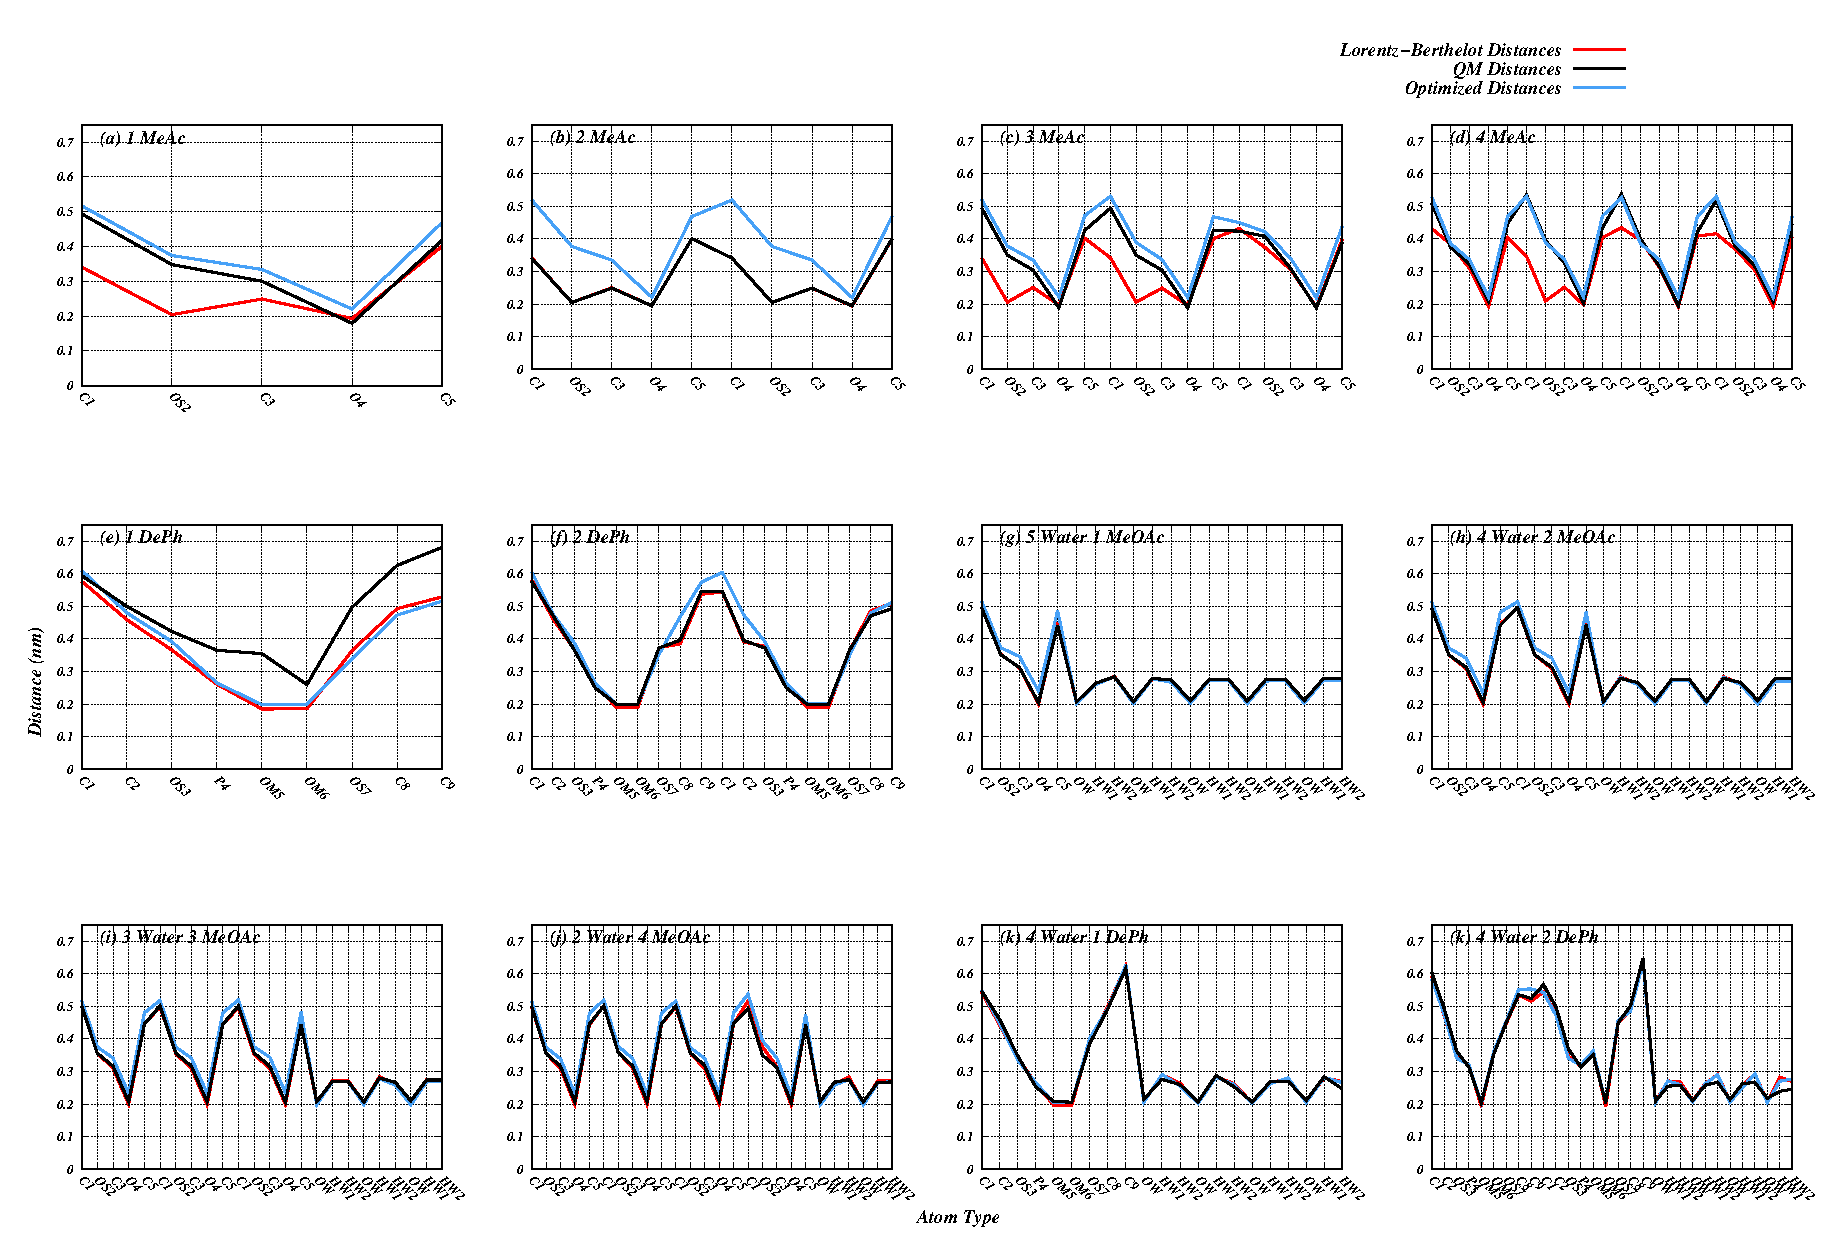
\includegraphics[width=\textwidth]{Figure_S1.eps}
\end{figure}
\clearpage
\begin{figure}
    \caption{Distances of all ligand atoms from ion, for each cluster. Lorentz-Berthelot parameters result in geometries that are very similar to the target data -- in general, the 
    optimized parameters result in the ion being slightly closer to the electronegative oxygens in each cluster.}
    \label{fig:distances}
    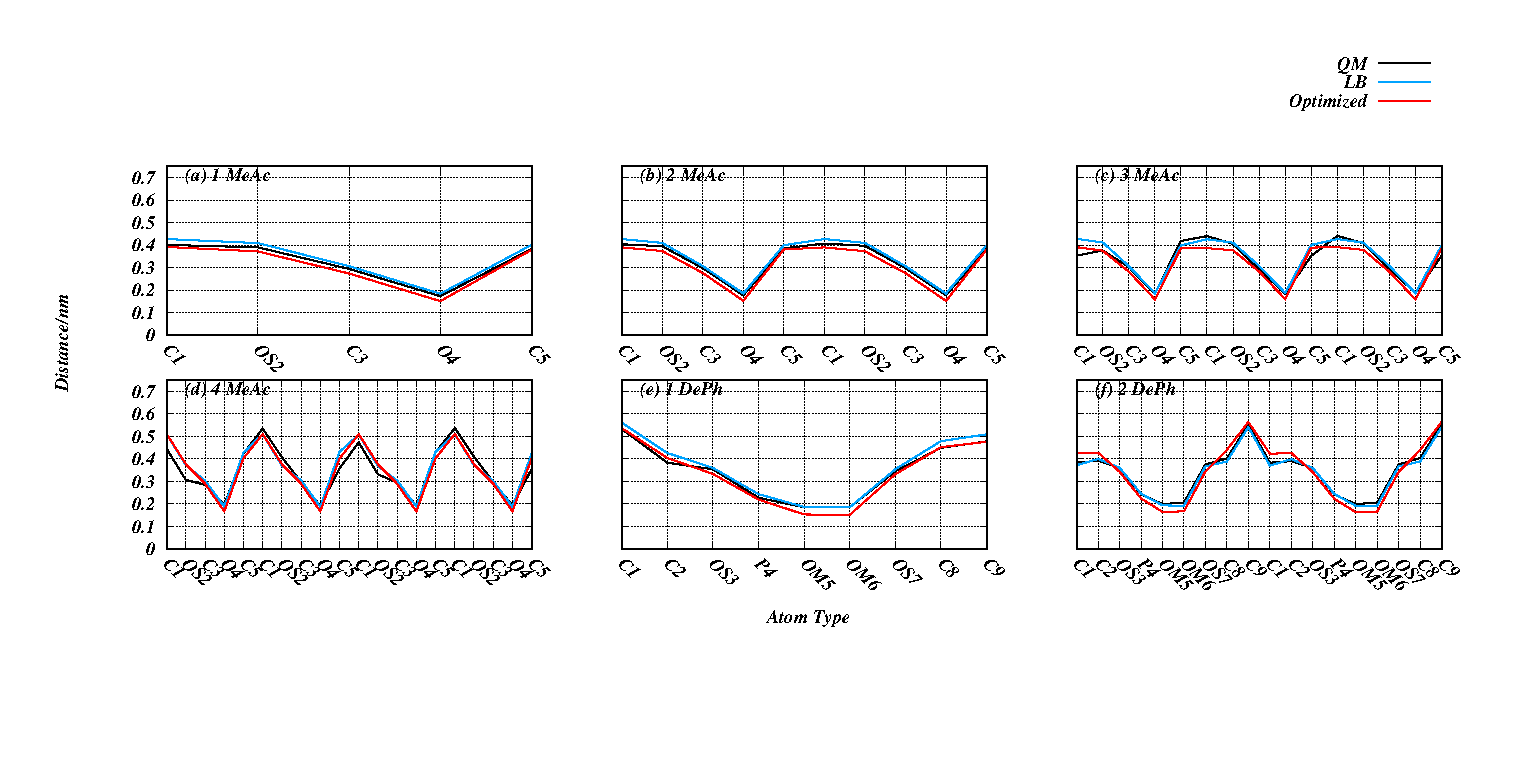
\includegraphics[width=\textwidth]{Figure_S2.eps}
\end{figure}
\ifdefined\COMPLETE
\else
\bibliography{refs}
\end{document}
\fi
